\section{Object Detection and Tracking}
\label{sec:introduction/section_a}

Object tracking problems can be categorized into Single Object Tracking (SOT) and Multiple Object Tracking (MOT). SOT tracks the single object over the sequence of digital images while MOT tracks the multiple objects. The following introduction of MOT has been explained well by \citeauthor{luo_multiple_2021} \cite{luo_multiple_2021}. SOT tracks a single object with a focus on appearance and motion models and MOT has common challenges with the single object case, but tracking with multiple objects will involve additional challenges to be solved. With the multiple objects case, the tracking system needs to determine the number of objects which could vary over the frames and preserve their identities. In this thesis work, we do not want to restrict to the single object and want to see the effects of compression on tracking with multiple objects, which is more general in reality.

\citeauthor{luo_multiple_2021} also explained the general categories of MOT. MOT initialization method can be grouped into Detection-Based Tracking and Detection-Free Tracking. Detection-Based Tracking involves an object detector to perform detections as initialization to the tracker for every image in a sequence and then the object tracker will assign unique identities to each detected object, in other words, performing data association of unique ID based on detected objects. Detection-Free Tracking will not involve object detector but requires other initialization methods such as inference that exploits rich appearance and motion information \cite{lin_detection-free_2016}. MOT processing method can be group into online tracking and offline tracking. As you can see in Fig.\ref{fig:mot_processing_mod}, online tracking performs data association of unique identities based on current and past observations while offline tracking does by future, current, and past observations as a batch. Type of output from MOT can also be stochastic or deterministic. The output of stochastic tracking varies every time you run the tracker while the output is fixed for the deterministic case.

\begin{figure}[htb]
  \centering
  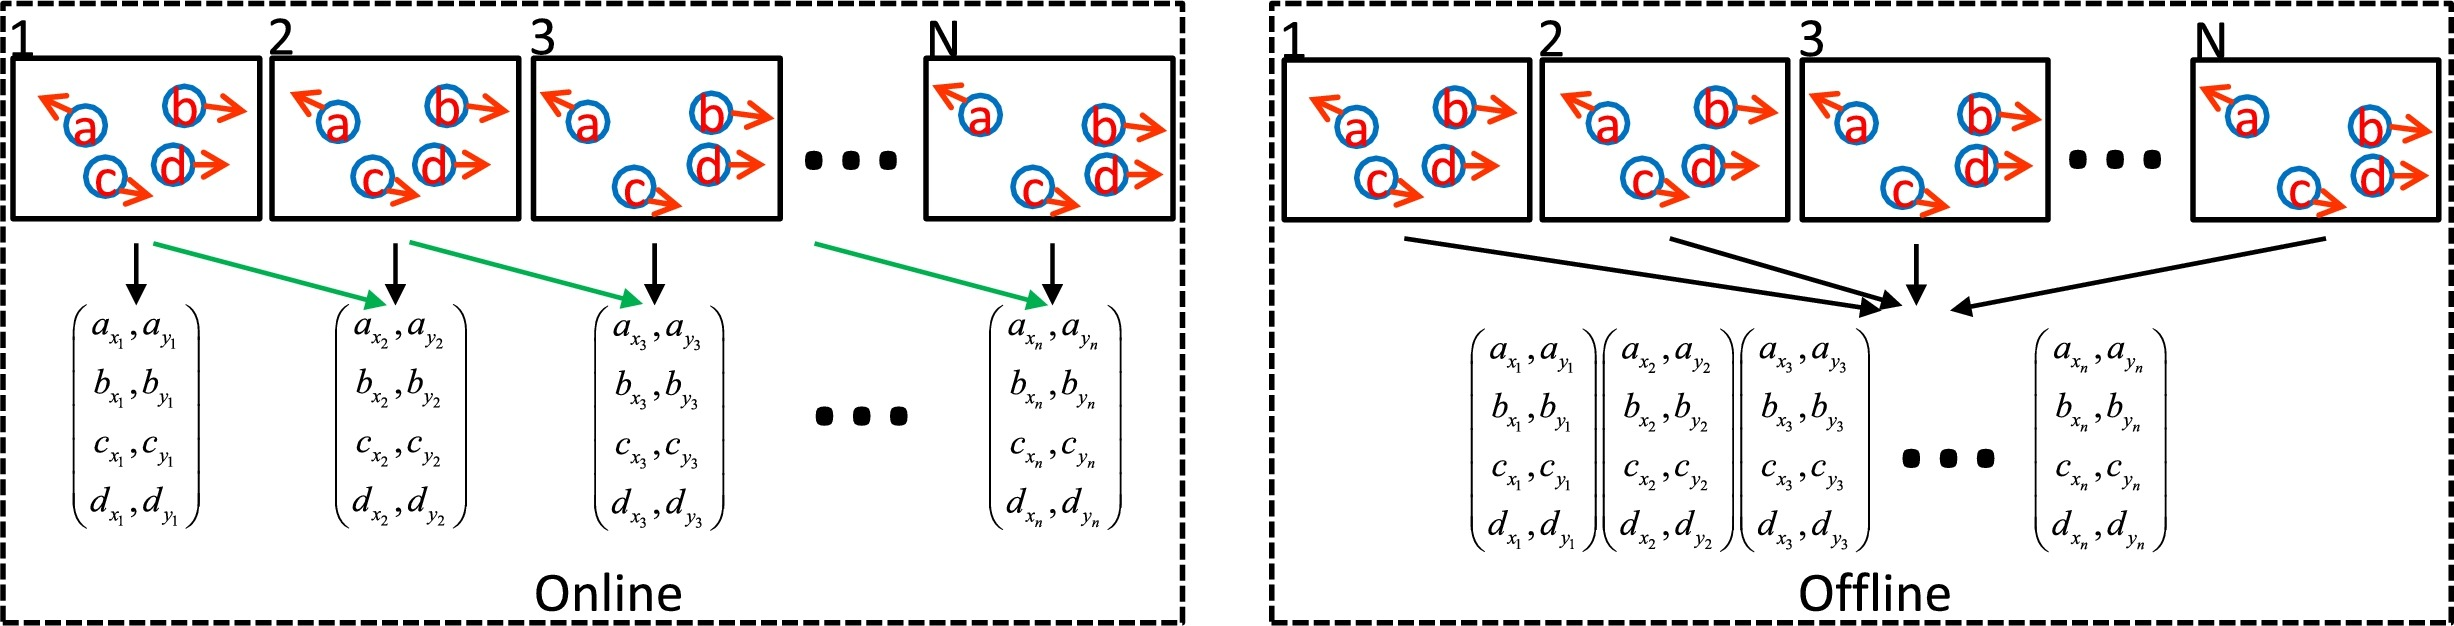
\includegraphics[width=0.8\linewidth]{img/mot_processing_mod.jpg}
  \caption[MOT Processing Methods]{%
    MOT Processing Methods. Left image shows online tracking that 
  }
  \label{fig:mot_processing_mod}
\end{figure}


For this thesis, we are using Detection-based Tracking and hence we will need an object detector before tracking. Object detection has been actively researched for the past 20 years in period and there are two period of stages the research have gone through according to \citeauthor{zou_object_2019} \cite{zou_object_2019}. The first stage is traditional detection method, which is hand-crafted method while the second stage is deep learning-based method. In 2012, the convolution neural network (CNN) regains its popularity since it is able to learn robost and high level feature of the image. The deep learning based method can be further broken down into two category; one-stage detection and two-stage detection. For two-stage detectors, the first stage generates the region of interest as a bounding box detection proposal and each region proposal is feed into CNN and classification and regression performed on each proposal as a second stage. Various two-stage deep learning-based method have been developed such as RCNN (Region Based Convolutional Neural Network), SPP-net (Spatial Pyramid Pooling network), Fast RCNN, Faster RCNN, FPN (Feature Pyramid Network), and Mask RCNN. As for one-stage detectors, the full image is feed into the single neural network and each bounding box as a region of interest is predicted by the network. The examples for the one-stage detector could be YOLO (You Only Look Once), SSD (Single-Shot Multibox Detection), and RetinaNet \cite{zou_object_2019} \cite{sultana_review_2020}.

\citeauthor{luo_multiple_2021} listed the examples of models used in multiple object tracker. There are appearance model that computes the affinity between the observations based on the visual cues and statistical measures, motion model that captures dynamic behaviour of objects such as linear and non-linear motion, interaction model that considers individual interaction in the social environment, exclusion model that utilizes constraint between objects or trajectories, occlusion handling model, and finally inference model that considers probability distribution of object states or approach based on the deterministic optimization.

Out of all possible ways to detect and track as listed above, we employed the YOLO v3 object detector with Simple Online Realtime Tracking (SORT). This solution is detection-based and online tracking with deterministic output and the detail is explained in the chapter \ref{chap:background}.
